\documentclass{tektonika}


\newcommand{\Title}{This is our mountanious title} % Manuscript title goes here

\newcommand{\shortTitle}{Our short mont title} % Short title for header goes here

\newcommand{\FirstAuthor}{Author et al.\xspace} % First author goes here. Leave blank if opting for blind review.

\newcommand{\AllAuthors}{A. Author\textsuperscript{1,2}*, \& 
	B. Author \textsuperscript{2} }
% Author list goes here, with affiliations defined. Corresponding author email address is defined in the same way. Leave blank if opting for blind review.

\newcommand{\Affiliation}{
	\textsuperscript{1}{School of Natural Sciences, University A, Ghana}\\
	\textsuperscript{2}{Institute for Rocks, University B, Nepal}
}


\newcommand{\CorrEmail}{{*}Corresponding author (e-mail: \url{anne.author@unia.edu.gh})}
\newcommand{\Year}{2022} % Year goes here
\newcommand{\vol}{1} % Volume goes here
\newcommand{\doi}{doi:00.0000/00000.00000} % doi here, when available




%%%%%%%%%%%%%%%%%%%%%%%%%%%%%%%%%%%%%%%%%%%%%%%%%%%%%%%%%%%%%%%%%%%%%%%%%%
% ARTICLES:  Regular, full research papers presenting original contributions that represent a key advance in scientific knowledge or understanding. A length under 10,000 words (excluding figure captions, texts in tables and references) and 20 figures/tables are preferred, albeit not enforced. Tektonika reserves the right to request the shortening of excessively long or detailed articles. Authors should include ‘Plain Language Summaries’ in articles.

% Figure sizes should not exceed 85x200 mm for single column figures or 175x200 mm for two column figures.

\begin{document}

\maketitle
\thispagestyle{firststyle}

\begin{abstract}
Abstract text here, and continues in the second paragraph. \\

More here, in a second paragraph. Hope you like our paper. 
\end{abstract}


\section{Introduction}
The main body of the text should go here.
\lipsum[1]

\begin{figure}[h!]\centering
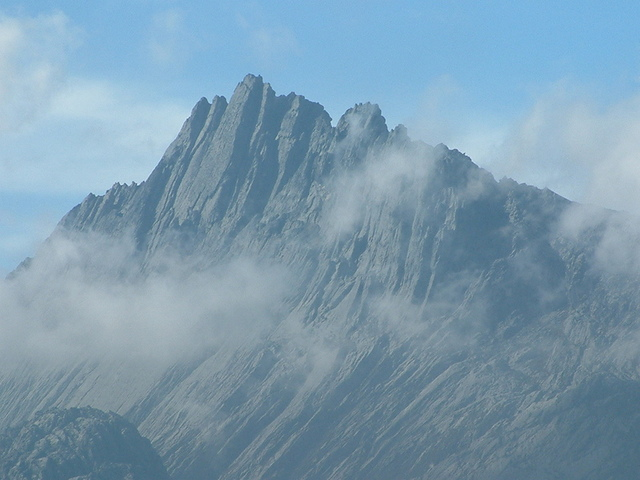
\includegraphics[width=0.5\textwidth]{Puncakjaya} 
\caption{Puncak Jaya. Photo by Alfindra Primaldhi (cc-by-2.0).}
\label{fig:1}
\end{figure}

\subsubsection{Sub-subsections appear like this}

Examples of citations: \citep{jordan1981},  \citet{staal2021a}, \citep[discussed by e.g.][]{staal2021a}. 


\section{Methods}
The main body of the text should go here.
\lipsum[1]




Equations are defined in the \{equation\} environment:
 \begin{equation}
\dot{\varepsilon} = A\sigma^{n} f_{H_{2}O}^{r} e^{({\frac{-Q}{RT}})}
\end{equation}

\section{Results}
The main body of the text should go here.
\lipsum[1]



\section*{Acknowledgements} % Please upload separately if opting for blind review.
We thank.


\section*{Author contributions} % Please upload separately if opting for blind review.
AA did this and BB did that. 

\section*{Data availability}
Output models in interoperability formats are available from \url{url_to_zenodo}. Code used to generate the results in this article is available from \url{url_to_github}, and achieved at \url{url_to_zenodo}. \\


This article is distributed under the terms of the Creative Commons Attribution 4.0 International Licence (CC BY 4.0), which permits unrestricted use, distribution, and reproduction in any medium, provided appropriate credit to the original author(s) and source, as well as link to the Creative Commons license, and indication of changes that were made.


\bibliography{ref} % a separate bibfile is required. Please upload this file along with the compiled manuscript and source file.

%%%%%%%%%%%%%%%%%%%%%%%%%%%%%%%%%%%%%%%%%%%%%%%%%%%%%%%%%%%%%%%%%%%%%%%%%%
\end{document}
